\chapter*{致读者}
\phantomsection
\addcontentsline{toc}{chapter}{致读者}

\begin{enumerate}
\def\labelenumi{\arabic{enumi}.}
\item
  本《数学原理》丛书从数学的开端讲起，并给出完整的证明。原则上，它并不要求读者具备任何专门的数学知识，而只要求对数学推理有一定的熟悉以及一定的抽象思维能力。不过，它特别是为那些至少已较好地掌握大学数学课程头一两年内容的读者而写的。
\item
  我们所选用的叙述方法是公理化的，并且通常从一般过渡到特殊。证明的需要使题材具有一种严格固定的顺序。因此，除非读者已经具备相当广博的数学知识，否则某些考虑的用处不会立即显现在他面前。
\item
  丛书分为若干卷，每卷又分为若干章。下面列出在法文版中已全部或部分出版的各卷。凡有英译本时，括号中给出相应的英文书名。在本卷中，引用一律指英文版（如果有的话），否则指法文版。
\end{enumerate}

Théorie des Ensembles (Theory of Sets) 记作 E (S)

Algèbre (Algebra) --- A (A)

Topologie Générale (General Topology) --- TG (GT)

Fonctions d'une Variable Réelle (Functions of a Real Variable) --- FVR (FRV)

Espaces Vectoriels Topologiques (Topological Vector Spaces) --- EVT (TVS)

Intégration (Integration) --- INT (INT)

(Commutative Algebra) --- AC (CA)

Variétés Différentielles et Analytiques --- VAR

(Lie Groups and Lie Algebras) --- LIE (LIE)

Théories Spectrales --- TS

在前六卷（按上述顺序）中，正文里的每一陈述都只假定已知那些已在同一章中讨论过的结果，或在按如下顺序排列的前面各章中讨论过的结果：S；A，第 I 至 III 章；GT，第 I 至 III 章；A，从第 IV 章起；GT，从第 IV 章起；FRV；TVS；INT。

从第七卷起，读者通常会在其中找到关于该卷与其他各卷之间逻辑关系的确切说明（前六卷总假定为已知）。

\begin{enumerate}
\def\labelenumi{\arabic{enumi}.}
\setcounter{enumi}{3}
\item
  不过，我们有时在正文中插入了一些例子，它们涉及读者可能已经知道、但在本丛书中尚未讨论的事实。这类例子置于两个星号之间：*\ldots*。大多数读者无疑会发现这些例子有助于理解正文。在另一些情形，*\ldots* 之间的段落所涉及的结果在本丛书的别处讨论。我们希望读者能够自行验证其中不存在任何恶性循环。
\item
  每一章的逻辑框架由该章的定义、公理和定理组成。这些是以后使用时主要应当记住的部分。较次要的结果以及那些容易由定理推出的结果，标以“命题”、“引理”、“推论”、“注记”等名称。初读时可以略去的那些部分以小号字排印。对特别重要的定理所作的评注，偶尔以“scholium（评注）”之名出现。
\end{enumerate}

为了避免令人生厌的重复，有时方便的做法是引入仅在某一章或某一章的某一节内有效的记号或缩写（例如，在只讨论交换环的一章中，“环”一词总是指“交换环”）。这类约定总会被明确指出，一般是在出现该约定的一章的开头。

\pandocbounded{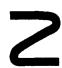
\includegraphics[keepaspectratio]{images/part001_c576909a.jpg}}

\begin{enumerate}
\def\labelenumi{\arabic{enumi}.}
\setcounter{enumi}{5}
\item
  正文中有一些段落旨在预先提醒读者谨防严重错误。这些段落用（“危险弯道”）记号在页边标出。
\item
  习题的目的，一方面是使读者能确信自己已经消化了正文，另一方面是使读者注意到那些在正文中没有位置却仍有意义的结果。最难的习题带有记号 ¶。
\item
  一般说来，我们遵循通行的术语，除非看来有充分理由偏离它。
\item
  我们特别致力于始终使用严格正确的语言而不牺牲简洁性。对于各种语言滥用，我们在正文中尽可能加以提醒；没有这类滥用，任何数学文本都有流于迂腐、甚至无法阅读的危险。
\item
  由于正文原则上是对一个理论的教条式陈述，它一般不包含对文献的引用。书目式引用汇集于历史注记之中。每篇历史注记后面所附的参考文献一般只包括那些对所述理论的演进曾起过最重要作用的书籍和原始论文。它绝不冒称在任何意义上是完备的。
\end{enumerate}

至于习题，我们一般不认为值得注明其出处，因为它们取自许多不同的来源（原始论文、教科书、习题集）。

\begin{enumerate}
\def\labelenumi{\arabic{enumi}.}
\setcounter{enumi}{10}
\tightlist
\item
  对本丛书某一部分的引用按如下方式给出：
\end{enumerate}

\begin{enumerate}
\def\labelenumi{\alph{enumi})}
\item
  若引用的是同一节（§）中陈述的定理、公理或定义，则按其编号引用。
\item
  若它们出现在同一章的另一节中，则在引用时同时注明该节。
\item
  若它们出现在同一卷的另一章中，则注明章与节。
\item
  若它们出现在另一卷中，则先注明该卷，用其书名的缩写表示。
\end{enumerate}

结果汇编以字母 R 引用；于是 S, R 表示“集合论的结果汇编”。

\chapter*{引言}
\phantomsection
\addcontentsline{toc}{chapter}{引言}

量的测度这一概念是根本性的，无论在日常生活（长度、面积、体积、重量）中，还是在实验科学（电荷、磁质量等）中都是如此。如此多种多样的量的“测度”的共同特征在于：对满足某些条件的每一部分空间联结一个数，使得对两个这样的部分（假定没有公共点）的并，对应于分别赋予它们各自的数之和（测度的可加性）(*)。此外，测度通常是一个正数，这就意味着它是被测的那部分空间的递增函数 (**)。另一方面可以注意到，在实际中人们几乎从不操心去指明哪些部分空间应当看成“可测的”；当然，在任何一种测度的数学理论中，都必须毫不含糊地解决这个问题；例如，在初等几何中定义多边形的面积或多面体的体积时，人们做的就是这件事；在所有这些情形，“可测”集的族自然必须满足：其中任意两个无公共点的集合的并也是“可测的”。

在上面大多数例子中，一部分空间的测度随其直径而趋于 0：按经典的说法，一个点“没有长度”，这就是说它含于长度任意小的区间之中，因而只能赋予它长度 0；这样的量的测度称为“弥散的”。然而，力学和物理学的发展引入了这样一类量的概念：对这类量，一个尺寸可忽略的物体仍可以具有不可忽略的测度：引力的或电的“点质量”，说实在的，它们在很大程度上是数学虚构，而不是严格意义上的实验概念。于是，在数学中人们被引向考虑如下定义的测度：对一个有限集的每一点 \(a_i\) ( \(1 \leqslant i \leqslant n\) )（记此有限集为 \(F\) ）附加一个数 \(m_i\) ，即它的“质量”或“重量”，而任一集合 \(A\) 的测度，就是质量 \(m_i\) 的和，这里点 \(a_i\) 属于 \(A\) 。

与测度概念紧密联系在一起的是加权和的概念。例如，考虑空间中有限多个（引力的或电的）质量 \(m_{i}\) ，它们置于点 \(a_{i}\) （坐标为 \(x_{i}, y_{i}, z_{i}\) ）处；这组质量施加于点 b（质量为 1，坐标为 \(\alpha, \beta, \gamma\) ）上的引力沿 Oz 方向的分量（例如）是（在适当选取的单位制下的）和式

\[
\sum_ {i} m _ {i} \frac {(z _ {i} - \gamma)}{r _ {i} ^ {3}},
\]

\(r_i^2 = (x_i - \alpha)^2 + (y_i - \beta)^2 + (z_i - \gamma)^2\) 是点 \(a_i\) 与 \(b\) 之间距离的平方。换句话说，我们考虑函数

\[
f (x, y, z) = \frac {z - \gamma}{\left((x - \alpha) ^ {2} + (y - \beta) ^ {2} + (z - \gamma) ^ {2}\right) ^ {3 / 2}}
\]

在每个点 \(a_{i}\) 处的值，把它乘以该点的“权重”，再把如此得到的 f 的“加权值”全部加起来。众所周知，这样的和式在力学中不断地出现：重心和惯性矩就是最著名的例子。

如果人们想要把“加权和”的概念从点质量的情形推广到每一点测度均为零的“弥散”测度的情形，就会遇到那个外表如此悖理、并催生了积分学的问题：如何给一个具有无穷多项、而每一项单独取出来都是零的“和”赋予意义。让我们再回到计算施加于一点上的引力的例子，其中吸引的质量“连续地分布”在整个体积 V 中。如果把 V 分解为有限个（两两不相交的）子集 \(V_{i}\) ，我们就假定 V 施加于点 b 上的引力沿 Oz 方向的分量等于各个 \(V_{i}\) 施加于 b 上的引力的分量之和。而如果每个 \(V_{i}\) 的直径都很小，连续函数 \(f(x,y,z)\) 在 \(V_{i}\) 中就变化很小，于是人们被引向把 \(V_{i}\) 所施加的引力近似地看成一个点质量所会施加的引力，该点质量等于质量 \(m_{i}\) （即 \(V_{i}\) 的质量），并置于点 \(a_{i}\) 处（该点任取于体积 \(V_{i}\) 之中）。于是人们被引向取“Riemann 和” \(\sum m_{i}f(x_{i},y_{i},z_{i})\) 作为所求数的近似值；为使这在数学观点上得到论证，自然必须证明当 \(V_{i}\) 的最大直径趋于 0 时这些近似值趋于一个极限，而这由函数 f 在 V 中的一致连续性容易得到（假定 V 是紧的且点 b 不在 V 中）。

众所周知，希腊人的“穷竭法”以及用于系统地计算平面图形面积与体积的“Cavalieri 原理”，都建立在一个类似的程序上，即把所考虑的面积与体积分解成“切片”；由此得到的“加权和”不是别的，正是积分 \(\int_{a}^{b} f(x) dx\) （参见第 IV 卷第 I--III 章的历史注记）。这里同样是 f 的一致连续性蕴涵着“Riemann 和”极限的存在性；更一般地，它蕴涵类似的和式 \(\sum_{i} f(\xi_{i})(g(x_{i+1}) - g(x_{i}))\)

\((x_{i} \leqslant \xi_{i} \leqslant x_{i+1})\) （其中只假定 g 是 \([a, b]\) 上的有界递增函数）时极限存在。这一极限记作 \(\int_{a}^{b} f(x) dg(x)\) ，称为 f 关于 g 的 Stieltjes 积分，它可以看作函数 f 关于测度 \(\mu\) 的“加权和”，该测度在半开区间 \([\alpha, \beta]\) 所成的集上由公式 \(\mu([\alpha, \beta]) = g(\beta+) - g(\alpha+)\) 定义；它不再像通常的积分概念那样与微分学紧密地联系在一起 (*)。经典的“二重”积分和“三重”积分分别联系于平面面积的度量与体积的度量，情形也是如此。然而，所有这些积分概念彼此之间的联系不仅在于它们的定义，还在于下述特征：直线、平面或三维空间中某个紧子集 K 上的连续数值函数 f 的“积分” \(\mu(f)\) ，是与 K 上的连续函数空间 \(\mathcal{C}(K)\) 的元素 f 相联系的一个数；于是 \(f \mapsto \mu(f)\) 是 \(\mathcal{C}(K)\) 到 R 中的映射（有时称为“泛函”），它是：\(1^{\circ} linear\) （也就是说，\(\mu(\alpha f + \beta g) = \alpha \mu(f) + \beta \mu(g)\) 对一切标量 \(\alpha, \beta\) 和一切连续函数 f, g 成立）；\(2^{\circ} positive\) （也就是说，\(\mu(f) \geqslant 0\) 对每个满足 \(f \geqslant 0\) 的连续函数 f 成立）。

值得注意的是，反过来，这两条性质就足以刻画区间 \([a,b]\) 上的 Stieltjes 积分（F. Riesz 定理）。之所以如此，是因为从连续函数积分的值出发，能够重新构造出产生该积分的测度。这相当于（如果我们把 \(\int_{a}^{b}f(x)dx\) 解释为平面图形的面积的话），在假定积分对连续函数为已知的前提下，去计算一个区间的特征函数的积分。换句话说，问题在于以适当的方式把泛函 \(\mu(f)\) 延拓到一个既包含 \(\mathcal{C}(K)\) 又大到足以包含各区间的特征函数的函数集上。

完成这一延拓有若干种方法；其中最有意思的方法之一求助于函数空间的概念。我们知道，在空间 \(\mathbf{R}^n\) 上，范数 \(\| \mathbf{x}\|_{\infty} = \sup_{1\leqslant i\leqslant n}|x_i|\) 与 \(\| \mathbf{x}\|_1 = \sum_{i=1}^{n}|x_i|\) 定义同一个拓扑。通过“从有限过渡到无穷”，人们被引向考虑连续函数空间 \(\mathcal{C}(\mathrm{K})\) （\(\mathrm{K} = [a,b]\) 是 \(\mathbf{R}\) 中的一个紧区间）上的范数 \(\| f\|_{\infty} = \sup_{x\in \mathrm{K}}|f(x)|\) 与 \(\| f\|_1 = \int_a^b |f(x)|dx\) （在 Stieltjes 积分的情形则取 \(\int_a^b |f|dg\) ）。但在这里，这两个范数所定义的拓扑是不同的，而且对第一个范数完备的空间 \(\mathcal{C}(\mathrm{K})\) （GT, X, §1, No. 6, Th. 2 的推论 1），对第二个范数不再完备。更确切地说，可以把 \(\mathcal{C}(\mathrm{K})\) 关于范数 \(\| f\|_1\) 的完备化的元素与未必连续的函数的类等同起来，于是积分的延拓就简单地通过把泛函 \(\mu(f)\) （它定义在 \(\mathcal{C}(\mathrm{K})\) 上）连续地延拓到该空间的完备化上来实现（这一程序的技术细节在第 IV 章中陈述）。当然，我们曾假定连续函数的积分是借助一个测度（用上面回顾过的“Riemann 和”程序）来定义的；为得到 F. Riesz 定理，必须按同样的方式操作，只是把范数定义为 \(\mu(|f|)\) ，其中 \(\mu(f)\) 是定义在 \(\mathcal{C}(\mathrm{K})\) 上的正线性形式。

我们刚才概述的延拓方法不仅导出 Riesz 定理，而且它还允许对由比区间的特征函数“不连续得多”的函数所组成的类定义积分；在考察作为“可积”函数的集合的特征函数时，它同时允许把起初只对区间给出的测度延拓到相应的集合上，办法是令 \(\mu(A) = \mu(\varphi_A)\) ；这一延拓当然保持了测度的可加性与正性这两条基本性质。

前面讨论的是直线上的 Stieltjes 积分，但延拓方法可以立即搬到定义在平面或空间中的测度上，或定义在曲线上或曲面上的测度上。更一般地，在分析这些证明时可以看出，它们实际上对定义在任意局部紧空间 X 上的连续函数所成的空间 \(\mathcal{H}(X)\) 上的每一个正线性形式都有效，这些连续函数中的每一个都在某个紧子集（依具体的函数而定）之外为零。

积分理论因而可以适用的这类空间自然包括数值空间 \(R^{n}\) 以及流形；它也包括离散空间（在离散空间上，积分理论与实数的可和族的理论合而为一 (GT, IV, §7)），还包括与 R 的区间相同的、或与有限集相同的紧空间的（有限或无穷）乘积；我们以后将看到，这类乘积上的测度理论在概率演算中起着重要的作用。

把测度概念延拓到一般的局部紧空间，这在局部紧群的理论中显得特别富有成效；一般地说，每当在拓扑代数中想要“从有限过渡到无穷”，也就是说，想要把出现有限和的纯代数程序推广到“求和”必须处理无穷多项的情形，积分的概念看来就是恰当的工具。例如，我们知道 (A, III, §2)，有限群 G（在域 \(\mathbf{R}\) 上）的代数的元素，是形如 \(s \mapsto \alpha(s)\) 的映射（即 G 到 \(\mathbf{R}\) 中的映射），其乘法规则为 \(\alpha * \beta = \gamma\) ，其中 \(\gamma\) 是由下式定义的函数

\[
\gamma (s) = \sum_ {t \in G} \alpha (t) \beta (t ^ {- 1} s).
\]

对任意的局部紧群 G，这一代数的一个看来自然的推广，是 G 到 R 中的那样一些映射所成的集，它们关于 G 上某个特殊的测度 \(\mu\) （“Haar 测度”）可积，而代数中的乘法由

\[
(f * g) (s) = \int f (t) g (t ^ {- 1} s) d \mu (t).
\]

此外，一旦走上这条路，人们很快就会因为只能“求和”取实值的函数而感到不便；在许多情形，懂得如何去定义定义在 X 上、取值于 R 上的拓扑向量空间（例如一个 Banach 空间或 Banach 空间上的算子空间）中的函数的积分，是有用的。人们可以确认，这一延拓容易实现，无需对积分理论作任何深刻的修改。

在上述概述中，我们让连续函数扮演了占优势的角色；自然要问：测度的概念是否真的本质地依赖于它在其上定义的集合 X 上一个拓扑的存在。对理论的细致考察表明完全不是这么回事，而且延拓方法同样适用于定义在向量空间 V 上的正线性形式 \(\mu(f)\) ，这里 V 由定义在任意集合 X 上的数值函数组成，只需对 V 和 \(\mu(f)\) 附加某些补充条件；当 V 是具有紧支集的连续函数所成的空间 \(\mathcal{K}(\mathrm{X})\) 时，这些条件自动满足，但它们在更一般的情形中也能满足。不过，这种更大的普遍性在某些方面是虚幻的：事实上可以证明，每个“抽象测度”在某种意义下都“同构”于（从连续函数出发）定义在一个适当的局部紧空间上的测度；另一方面，大多数应用所涉及的集合 X 都带有在该问题中自然出现的拓扑；因此，直到第 IX 章，我们将只研究定义在局部紧空间上的测度。

前两章是本理论的预备篇章：它们致力于证明一些对延拓具有根本意义的不等式，并研究某些序向量空间，即 Riesz 空间，这些空间在后面的若干问题中起着重要的作用。

局部紧空间上的测度概念在第 III 章中定义；我们以 Riesz 定理为出发点，于是该定理在这里成为一个定义：连续函数的积分先于集合的测度得到定义，即定义为 \(\mathcal{K}(\mathrm{X})\) 上的一个正线性形式。这种表述方式具有某些技术上的优点（特别是因为连续函数构成一个向量空间，而集合的特征函数却不然）；此外，正是在 \(\mathcal{K}(\mathrm{X})\) 上的泛函的形式下，积分在大量问题中自然地出现。最后，\(\mathcal{K}(\mathrm{X})\) 上两个正线性形式之差（我们仍称之为 X 上的测度）可以刻画为 \(\mathcal{K}(\mathrm{X})\) 上满足某些连续性条件的线性形式；这样，积分理论一方面联系于拓扑向量空间中的一般对偶理论（参见第 V 卷），另一方面联系于分布理论，分布推广了测度概念的某些方面，我们将在随后的一卷中陈述它。

第 IV 章专门讨论积分的延拓；在那里同时定义了可积函数与集合的测度，还定义了函数空间 \(L^{p}\) ，它们在应用中的重要性是可观的；那里还说明了，可测函数概念的引入如何导出便于使用的可积性判别法。

在其后两章中将看到，可测函数又如何作为“密度”出现，使得能从一个给定的测度出发，在空间 X 上定义新的测度。这项研究特别导出 \(L^{p}\) 空间对偶理论中的若干重要结果，它还与向量测度的概念相联系；在最有利的情形，向量测度可以归结为向量值函数（关于一个正测度）的积分理论。

我们还将展开可以视为积分学创立者们所引入的平面面积与体积“切片分解”思想的现代极致的内容：在一定条件下，空间 X 上的一个测度可以分解为一个“和”，和中的每个测度都由空间 X 的一条“切片”（也就是关于某个关系 R 的一个等价类）所承载；此外，这样的分解使得能够通过先“在每条切片上”积分、再（关于一个适当的测度）对商空间 X/R 上由此得到的函数积分，来计算一个函数关于原来那个测度的积分（这是对指标取遍一个乘积集的族的和式的“二重求和”的一个推广）。

第 VII 章专门研究局部紧群上的 Haar 测度，它在相差一个标量倍数的意义下，由在群的每个左平移下不变这一性质所刻画。

第 VIII 章陈述测度的卷积，这一概念在现代泛函分析中起着头等重要的作用。

第 IX 章专门讨论未必局部紧的 Hausdorff 拓扑空间中的积分，特别是局部凸向量空间中的积分；这特别使得 Fourier 变换的理论能够延拓到后面这类空间。开头几节所选的叙述方式，在于尽可能化归为前面各章中已处理过的紧空间的情形。

\chapter{凸性不等式}

\section{凸性的基本不等式}

设 X 是一个集；在向量空间 \(R^{X}\) （由定义在 X 上的全体有限数值函数 \(^{1}\) 组成）中，设 P 是 X 上全体正实值函数所成的集。另一方面，设 M 是定义在 P 上的一个数值函数 \(^{2}\) ，有限与否皆可，取值 \(\geqslant0\) ，并且满足：

\(1^{\circ} M(0) = 0\) ，且 \(M\) 是正齐次的，也就是说，\(M(\lambda f) = \lambda M(f)\) 对每个实数 \(\lambda > 0\) 成立。

\(2^{\circ} M\) 在 P 中递增，换言之，关系 \(f \leqslant g\) 蕴涵 \(M(f) \leqslant M(g)\) 。

\(3^{\circ} M\) 在 P 中是凸的，换言之，它 (TVS, II, §2, No. 8) 满足关系 \(M(f + g) \leqslant M(f) + M(g)\) 。

例. --- 设 X 是一个有限集，例如 N 的区间 \([1,n]\) ；用 \(x_{i}\) ( \(1 \leqslant i \leqslant n\) ) 表示向量 \(x \in R^{n}\) 的坐标，则函数 \(M_{1}(\mathbf{x}) = \sum_{i=1}^{n} x_{i}\) 与 \(M_{\infty}(\mathbf{x}) = \sup_{1 \leqslant i \leqslant n} x_{i}\) 在由坐标 \(\geqslant 0\) 的向量 x 所组成的集 P 中满足前述条件。

注. --- 设 S 是含于 P 中的一个带顶点的凸锥（也就是说，一个满足 \(S + S \subset S\) 与 \(\lambda S \subset S\) （对 \(\lambda \geqslant 0\) ）的集；参见 TVS, II, §2, No. 4）；设 M 是定义在 S 上、取值 \(\geqslant 0\) 的数值函数（有限与否皆可），且在 S 中满足上述条件 \(1^{\circ}\) 、\(2^{\circ}\) 与 \(3^{\circ}\) 。那么 M 可以延拓到整个集 P 上，并使延拓后的函数（我们仍记作 M）满足同样的条件：对每个函数 \(f \in P\) ，令 \(M(f) = +\infty\) ，如果不存在任何函数 \(g \in S\) 使得 \(f \leqslant g\) ；而在相反的情形，令 \(M(f) = \inf_{g \in S, f \leqslant g} M(g)\) ；如此即

可完成延拓。这一程序将在第 IV 章 §1 中用来定义正函数的上积分。

命题 1. --- 设 \(\varphi(t_{1}, t_{2}, \ldots, t_{n})\) 是一个有限数值函数，对 \(t_{i} \geqslant 0\) ( \(1 \leqslant i \leqslant n\) ) 有定义且连续，并满足：

\(1^{\circ}\) 关系 \(t_i > 0\) \((1\leqslant i\leqslant n)\) 蕴涵 \(\varphi (t_1,t_2,\dots ,t_n) > 0\) ；

\(2^{\circ}\) 函数 \(\varphi\) 是正齐次的；

\(3^{\circ}\) 集 \(\mathbf{K} \subset \mathbf{R}^{n}\) （由关系 \(t_{i} \geqslant 0\) ( \(1 \leqslant i \leqslant n\) ) 及 \(\varphi(t_{1}, t_{2}, \ldots, t_{n}) \geqslant 1\) 定义）是凸的。

在这些条件下，若 \(f_1, f_2, \ldots, f_n\) 是 \(n\) 个有限函数 \(\geqslant 0\) ，定义在 \(X\) 上，且使得 \(M(f_i) < +\infty\) 对 \(1 \leqslant i \leqslant n\) 成立，则

\[
M \left(\varphi \left(f _ {1}, f _ {2}, \dots , f _ {n}\right)\right) \leqslant \varphi \left(M \left(f _ {1}\right), M \left(f _ {2}\right), \dots , M \left(f _ {n}\right)\right).\tag{1}
\]

由 Hahn-Banach 定理 (TVS, II, §5) 可知，K 是 n 个半空间 \(t_{i} \geqslant 0\) ( \(1 \leqslant i \leqslant n\) ) 与一族闭半空间 \((\mathrm{U}_{\iota})_{\iota \in \mathrm{I}}\) 的交，其中 \(U_{\iota}\) 由形如下式的关系定义

\[
\alpha_ {\iota 1} t _ {1} + \alpha_ {\iota 2} t _ {2} + \dots + \alpha_ {\iota n} t _ {n} - \beta_ {\iota} \geqslant 0,\tag{2}
\]

其中诸 \(\alpha_{\iota k}\) 不全为零。根据假设，若 \(\mathbf{t}=(t_{i})\) 满足 \(t_{i}>0\) （对 \(1\leqslant i\leqslant n\) ），则 \(\varphi(t_{1},\ldots,t_{n})>0\) ，因此存在 \(\lambda_{0}>0\) ，使得关系 \(\lambda\geqslant\lambda_{0}\) 蕴涵 \(\lambda t\in K\) ；这表明，对每个 \(\iota\in I\) ，关系 \(t_{i}\geqslant0\) ( \(1\leqslant i\leqslant n\) ) 蕴涵 \(\alpha_{\iota1}t_{1}+\cdots+\alpha_{\iota n}t_{n}\geqslant0\) ，从而 \(\alpha_{\iota k}\geqslant0\) 对 \(1\leqslant k\leqslant n\) 成立；于是显然，K 也是诸半空间 \(t_{i}\geqslant0\) ( \(1\leqslant i\leqslant n\) ) 与诸 \(U_{\iota}\) （即使 \(\beta_{\iota}\geqslant0\) 的那些）的交；此外，由于原点不属于 K，至少存在一个指标 \(\iota\) 使得 \(\beta_{\iota}>0\) 。

现在设 C 是 \(R^{n+1}\) 中由关系 \(t_{i} \geqslant 0\) ( \(1 \leqslant i \leqslant n + 1\) ) 与 \(t_{n+1} \leqslant \varphi(t_{1}, t_{2}, \ldots, t_{n})\) 所定义的凸锥（即在 \(R^{n+1}\) 中由凸集 \(K \times \{1\}\) 生成的凸锥的闭包）；立即可以看出，C 也可以由关系 \(t_{i} \geqslant 0\) ( \(1 \leqslant i \leqslant n + 1\) ) 以及

\[
\beta_ {\iota} t _ {n + 1} \leqslant \alpha_ {\iota 1} t _ {1} + \dots + \alpha_ {\iota n} t _ {n} \quad (\iota \in \mathrm{I}, \beta_ {\iota} \geqslant 0).\tag{3}
\]

因此，对每个 \(x \in X\) ，我们有

\[
\beta_ {\iota} \varphi (f _ {1} (x), \dots , f _ {n} (x)) \leqslant \alpha_ {\iota 1} f _ {1} (x) + \dots + \alpha_ {\iota n} f _ {n} (x)\tag{4}
\]

对一切 \(\iota \in I\) 成立。对每个指标 \(\iota\) （它满足 \(\beta_{\iota} > 0\) ），由 (4) 式及关于 \(M\) 的假设可知 \(M(\varphi(f_1, f_2, \ldots, f_n))\) 有限，且

\[
\beta_ {\iota} M \left(\varphi \left(f _ {1}, f _ {2}, \dots , f _ {n}\right)\right) \leqslant \alpha_ {\iota 1} M \left(f _ {1}\right) + \alpha_ {\iota 2} M \left(f _ {2}\right) + \dots + \alpha_ {\iota n} M \left(f _ {n}\right),
\]

而当 \(\beta_{\iota} = 0\) 时，这一关系也以显然的方式成立。这样一

来即可看出，坐标为

\[
M (f _ {1}), M (f _ {2}), \dots , M (f _ {n}), M (\varphi (f _ {1}, f _ {2}, \dots , f _ {n}))
\]

的点属于 C，这就证明了本命题。

\section{Hölder 不等式与 Minkowski 不等式}

在本小节及下一小节中，X 与 P 的含义与第 1 小节中的相同，M 表示定义在 P 上且满足第 1 小节所列条件的函数。

命题 2. --- 设 \(\alpha\) 与 \(\beta\) 是两个数，满足 \(0 < \alpha < 1\) ，\(0 < \beta < 1\) ，\(\alpha + \beta = 1\) 。若 \(f\) 与 \(g\) 是定义在 X 上的两个有限函数 \(\geqslant 0\) ，且 \(M(f)\) 与 \(M(g)\) 有限，则

\[
M (f ^ {\alpha} g ^ {\beta}) \leqslant (M (f)) ^ {\alpha} (M (g)) ^ {\beta}\tag{5}
\]

（Hölder 不等式）。

由命题 1，问题归结为证明：在 \(\mathbf{R}^2\) 中，由关系 \(t_1 \geqslant 0\) 、\(t_2 \geqslant 0\) 、\(t_1^\alpha t_2^\beta \geqslant 1\) 所定义的集是凸的，或者等价地 (FRV, I, §4, No. 1, Def. 1)，证明函数 \(u(t) = t^{-\alpha/\beta}\) 在 \(0 < t < +\infty\) 上是凸的。而若令 \(r = \alpha/\beta\) ，我们有 \(\mathrm{D}^2 u(t) = r(r + 1)t^{-r - 2}\) ，且由于 \(r > 0\) ，\(\mathrm{D}^2 u(t) > 0\) 在 \(]0, +\infty[\) 上成立，这就证明了本命题 (FRV, I, §4, No. 4, Prop. 8 的推论)。

推论. --- 设 \(\alpha_{i}\) ( \(1 \leqslant i \leqslant n\) ) 是 n 个数 \(\geqslant 0\) ，满足 \(\sum_{i=1}^{n} \alpha_{i} = 1\) ；又设 \(f_{i}\) ( \(1 \leqslant i \leqslant n\) ) 是定义在 X 上的 n 个函数 \(\geqslant 0\) ，使得 \(M(f_{i})\) 对 \(1 \leqslant i \leqslant n\) 有限。在这些条件下，

\[
M \left(f _ {1} ^ {\alpha_ {1}} f _ {2} ^ {\alpha_ {2}} \dots f _ {n} ^ {\alpha_ {n}}\right) \leqslant \left(M (f _ {1})\right) ^ {\alpha_ {1}} \left(M (f _ {2})\right) ^ {\alpha_ {2}} \dots \left(M (f _ {n})\right) ^ {\alpha_ {n}}.\tag{6}
\]

我们只需限于对每个 i 都有 \(\alpha_{i} > 0\) 的情形。只需对 n 作归纳论证，把不等式 (5) 应用于数 \(\alpha = \alpha_{1}\) 与 \(\beta = \sum_{i=2}^{n} \alpha_{i}\) ，并应用于函数 \(f = f_{1}\) 与 \(g = (f_{2}^{\alpha_{2}} f_{3}^{\alpha_{3}} \cdots f_{n}^{\alpha_{n}})^{1/\beta}\) 。

命题 3. --- 设 p 是一个实数 \(\geqslant 1\) 。若 f 与 g 是定义在 X 上的两个有限函数 \(\geqslant 0\) ，则

\[
\left(M \big ((f + g) ^ {p} \big)\right) ^ {1 / p} \leqslant \left(M (f ^ {p})\right) ^ {1 / p} + \left(M (g ^ {p})\right) ^ {1 / p}\tag{7}
\]

（Minkowski 不等式）。

我们只需限于 \(M(f^{p})\) 与 \(M(g^{p})\) 均有限的情形。由命题 1，问题归结为证明 \(R^{2}\) 中由关系 \(t_{1} \geqslant 0\) 、\(t_{2} \geqslant 0\) 、\(t_{1}^{1/p} + t_{2}^{1/p} \geqslant 1\) 所定义的集是凸的，或者等价地，证明函数 \(u(t) = (1 - t^{1/p})^{p}\) 在 \(0 \leqslant t \leqslant 1\) 上是凸的。而我们有

\[
\mathrm{D} ^ {2} u (t) = \left(1 - \frac {1}{p}\right) t ^ {1 / p - 2} (1 - t ^ {1 / p}) ^ {p - 2} \geqslant 0
\]

对 \(0 < t \leqslant 1\) 成立，由此即得本命题。

\section{\texorpdfstring{半范数 \(\mathbf{N}_p\)}{半范数 N sub p}}

设 \(p\) 是一个实数 \(\geqslant 1\) ，又设 \(\mathcal{F}^p(\mathrm{X},M)\) 是这样的有限数值函数 \(f\) （定义在 \(\mathrm{X}\) 上）所成的集：它使 \(M(|f|^p)\) 为有限。显然，若 \(g\) 是属于 \(\mathcal{F}^p(\mathrm{X},M)\) 的一个函数且 \(|f| \leqslant |g|\) ，则 \(f\) 也属于 \(\mathcal{F}^p(\mathrm{X},M)\) ；这一注记连同 Minkowski 不等式表明，\(\mathcal{F}^p(\mathrm{X},M)\) 中两个函数之和也属于此集；再注意到 \(M\) 是正齐次的，便知 \(\mathcal{F}^p(\mathrm{X},M)\) 是空间 \(\mathbf{R}^{\mathrm{X}}\) （即定义在 \(\mathrm{X}\) 上的一切有限数值函数所成的空间）的一个向量子空间。

对每个数 \(p > 0\) 及每个有限数值函数 \(f\) （定义在 \(X\) 上），令

\[
\mathrm{N} _ {p} (f) = \left(M (| f | ^ {p})\right) ^ {1 / p};
\]

则有 \(\mathrm{N}_p(\lambda f) = |\lambda |\mathrm{N}_p(f)\) 对每个标量 \(\lambda\) 成立；此外，若 \(p \geqslant 1\) ，则由 (7)，

\[
\mathrm{N} _ {p} (f + g) \leqslant \mathrm{N} _ {p} (f) + \mathrm{N} _ {p} (g),\tag{8}
\]

这就证明 \(N_{p}\) 是向量空间 \(\mathcal{F}^{p}(X,M)\) 上的一个半范数 (TVS, II, §1)。

命题 4. --- 设 p 与 q 是两个实数 \textgreater{} 0 ，并令 \(1/r = 1/p + 1/q\) 。对定义在 X 上的任意有限数值函数 f, g，

\[
\mathrm{N} _ {r} (f g) \leqslant \mathrm{N} _ {p} (f) \mathrm{N} _ {q} (g)\tag{9}
\]

只要 \(\mathrm{N}_p(f)\) 与 \(\mathrm{N}_q(g)\) 有限。

事实上，关系式 (9) 可以写成

\[
M (| f | ^ {r} | g | ^ {r}) \leqslant \bigl (M (| f | ^ {p}) \bigr) ^ {r / p} \bigl (M (| g | ^ {q}) \bigr) ^ {r / q},
\]

这不过是把 Hölder 不等式 (5) 应用于数 \(\alpha = r / p\) 与 \(\beta = r / q\) 以及函数 \(|f|^p\) 与 \(|g|^q\) 所得的结果。

推论. --- 假设 \(M(1) = 1\) ；那么，对每个定义在 X 上的有限数值函数 f，映射 \(p \mapsto \mathrm{N}_{p}(f)\) 在 {]}0, +∞{[} 上是递增的。

把不等式 (9) 应用于 g = 1 的情形，我们看到，\(\mathrm{N}_{r}(f) \leqslant \mathrm{N}_{p}(f)\) 对一切 q \textgreater{} 0 成立；既然由 \(1/r = 1/p + 1/q\) 所定义的数 r 跑遍使 0 < r < p 成立的数集（这里 q 跑遍 \textgreater{} 0 的数集），推论便得到证明。

命题 5. --- 对每个定义在 X 上的有限数值函数 f，1/p (p \textgreater{} 0) 的值中使 \(\mathrm{N}_{p}(f)\) 为有限者所成的集 I 或为空集，或为一个区间；若 I 不缩为一点，则映射 \(\alpha \mapsto \log \mathrm{N}_{1/\alpha}(f)\) 或在 I 上是凸的，或在 I 的内部恒等于 \(-\infty\) 。

设 r 与 s 是两个不同的数 \textgreater{} 0 ，使得 1/r 与 1/s 属于 I；问题归结为证明：若

\[
{\frac {1}{p}} = {\frac {t}{r}} + {\frac {1 - t}{s}},
\]

其中 \(0 < t < 1\) ，则

\[
\log \mathrm{N} _ {p} (f) \leqslant t \cdot \log \mathrm{N} _ {r} (f) + (1 - t) \log \mathrm{N} _ {s} (f),\tag{10}
\]

或者等价地，

\[
\mathrm{N} _ {p} (f) \leqslant \left(\mathrm{N} _ {r} (f)\right) ^ {t} \left(\mathrm{N} _ {s} (f)\right) ^ {1 - t},\tag{11}
\]

由 \(N_{p}\) 的定义，这一关系式可以写成

\[
M (| f | ^ {p}) \leqslant \left(M (| f | ^ {r})\right) ^ {t p / r} \left(M (| f | ^ {s})\right) ^ {(1 - t) p / s}.\tag{12}
\]

令 \(\alpha = tp / r\) ，我们有 \(1 - \alpha = (1 - t)p / s\) ，这由把 \(p\) 定义为 \(t, r, s\) 的函数的那个关系式得出；从而 \(p = \alpha r + (1 - \alpha)s\) 。于是 Hölder 不等式给出

\[
M \big (| f | ^ {r \alpha} | f | ^ {s (1 - \alpha)} \big) \leqslant \big (M (| f | ^ {r}) \big) ^ {\alpha} \big (M (| f | ^ {s}) \big) ^ {1 - \alpha},
\]

这正好就是不等式 (12)。

\chapter*{习题}
\phantomsection
\addcontentsline{toc}{chapter}{习题}

\begin{enumerate}
\def\labelenumi{\arabic{enumi})}
\item
  在第 1 小节的假设下，试证：X 上使 \(M(|f|)\) 为有限的有界函数所成的集是 \(\mathbf{R}^X\) 的一个子代数 A，而 X 上使 \(M(|f|) = 0\) 的有界函数所成的集是 A 中的一个理想。此外，若 \(M(1)\) 有限，试证：当 A 赋以 X 上的一致收敛拓扑时，映射 \(f \mapsto M(f)\) 是连续的。
\item
  设 X 是 R 中的区间 \([0, +\infty[\) ，S 是由定义在 X 上且在 X 上满足 \(0 \leqslant f(x) \leqslant kx\) 的函数（这里 k \textgreater{} 0 是一个依赖于 f 的有限数）所构成的凸锥。令 \(M(f) = 0\) （对 \(f \in S\) ）；而对定义在 X 上而不属于 S 的每个正函数 f，令 \(M(f) = +\infty\) 。试证 M 满足第 1 小节的条件，且 \(M(x) = 0\) ，且 \(M(x^{r}) = +\infty\) 对每个不等于 1 的数 r \textgreater{} 0 成立。
\item
  给出一个例子，其中 \(X\) 是一个二元素集，\(N sub p(\mathbf{x})\) 对每个 \(p > 0\) 及每个 \(\mathbf{x} \in \mathbf{R}^2\) 有限，但存在 \(p\) 的某些值，使映射 \(p \mapsto N sub p(\mathbf{x})\) 在这些值处不可微。
\item
  由几何平均不等式导出不等式 (6)
\end{enumerate}

\[
z _ {1} ^ {\alpha_ {1}} z _ {2} ^ {\alpha_ {2}} \dots z _ {n} ^ {\alpha_ {n}} \leqslant \alpha_ {1} z _ {1} + \dots + \alpha_ {n} z _ {n} \quad (\text {where} \sum_ {i = 1} ^ {n} \alpha_ {i} = 1)
\]

(FRV, III, §1, No. 1, Prop. 2)。（可化为 \(M(f_i) = 1\) 对 \(1 \leqslant i \leqslant n\) 成立的情形。）

\begin{enumerate}
\def\labelenumi{\arabic{enumi})}
\setcounter{enumi}{4}
\tightlist
\item
  设 \(\alpha\) 是一个实数 \(>1\) ，并令 \(\beta = 1 - \alpha < 0\) 。设 \(g\) 是定义在 X 上的一个有限函数，使得 \(g(x) > 0\) 对一切 \(x \in X\) 成立，且 \(M(g) > 0\) ；试证：对每个定义在 X 上的有限函数 \(f \geqslant 0\) （它使 \(M(f)\) 为有限），
\end{enumerate}

\[
M (f ^ {\alpha} g ^ {\beta}) \geqslant (M (f)) ^ {\alpha} (M (g)) ^ {\beta}
\]

（适当地应用 Hölder 不等式）。

\begin{enumerate}
\def\labelenumi{\arabic{enumi})}
\setcounter{enumi}{5}
\tightlist
\item
  由 Hölder 不等式导出 Minkowski 不等式（借助 Hölder 不等式为 \(M(f(f + g)^{p-1})\) 找一个上界）。若假定 \(M(f + g) = M(f) + M(g)\) 对每对函数 \(f, g\) （它们定义且 \(\geqslant 0\) 于 \(X\) 上）成立，则类似地由习题 5 可导出不等式
\end{enumerate}

\[
\left(M \big ((f + g) ^ {p} \big)\right) ^ {1 / p} \geqslant \left(M (f ^ {p})\right) ^ {1 / p} + \left(M (g ^ {p})\right) ^ {1 / p}
\]

在下列情形中：

\begin{enumerate}
\def\labelenumi{\alph{enumi})}
\tightlist
\item
  \(0 < p < 1\) ，\(f\) 与 \(g\) 是定义在 X 上的有限函数 \(\geqslant 0\) ，使得 \(f(x) + g(x) > 0\) 对一切 \(x \in X\) 成立，且 \(M(f^p)\) 与 \(M(g^p)\) 有限；b) \(p < 0\) ，\(f\) 与 \(g\) 是定义在 X 上的有限函数，使得 \(f(x) > 0\) 且 \(g(x) > 0\) 对一切 \(x \in X\) 成立，\(M(f^p)\) 与 \(M(g^p)\) 有限，且 \(M((f + g)^p) > 0\) 。
\end{enumerate}

\chapter*{历史注记}
\phantomsection
\addcontentsline{toc}{chapter}{历史注记}

（注意 --- 罗马数字指本注记末尾的参考文献。）

两个正量的算术平均与几何平均的概念可追溯到古代，特别是毕达哥拉斯学派曾把它们作为其喜爱的论题之一。这两个平均之间的不等式 \(\sqrt{ab} \leqslant \frac{1}{2}(a + b)\) 很可能也为他们所熟知；无论如何，Euclid 在与两数之和给定时使其乘积最大的问题相联系时证明了它。看来人们要等到相当晚的 1729 年，才由 MacLaurin 明确陈述了这一问题向 n 个数的推广以及相应的不等式（尽管比这困难得多的极值问题早在很久以前就已被研究过）。

从 18 世纪末起，其他一些类似的不等式出现在分析与几何中。例如，1789 年，Lhuilier 解决了与不等式

\[
\sqrt {\left(\sum_ {k = 1} ^ {n} a _ {k}\right) ^ {2} + \left(\sum_ {k = 1} ^ {n} b _ {k}\right) ^ {2}} \leqslant \sum_ {k = 1} ^ {n} \sqrt {a _ {k} ^ {2} + b _ {k} ^ {2}};
\]

相联系的一个几何最大值问题；Cauchy 在 1821 年证明了

\[
\left(\sum_ {k = 1} ^ {n} a _ {k} b _ {k}\right) ^ {2} \leqslant \left(\sum_ {k = 1} ^ {n} a _ {k} ^ {2}\right) \left(\sum_ {k = 1} ^ {n} b _ {k} ^ {2}\right)
\]

Hölder 不等式的特殊情形；Buniakowsky 于 1859 年、H. A. Schwarz 于 1885 年把 Cauchy 不等式推广到了积分。

然而，直到 19 世纪末，凸性不等式才成为系统研究的对象。O. Hölder 于 1888 年 (I) 在这个问题中引入了单变量凸函数的思想：他从 \(\log x\) 的凹性出发得到了几何平均不等式；把同样的思想应用于函数 \(x^{r}\) ，他证明了以他的名字命名的不等式，而 L. J. Rogers 在一年之前已经从几何平均不等式出发得到了这一不等式（参见习题 4）。至于 Minkowski 不等式，则由后者于 1896 年（对有限和）在与他关于“数的几何”的著名工作 ((II), pp. 115-117) 的联系中给出证明；虽然凸性思想（对任意多个变量的函数而言）是这项工作的基本概念之一，令人相当奇怪的是，Minkowski 竟未注意到他的不等式可以由 Hölder 方法应用于 \((1 + x^{r})^{1 / r}\) 而得到（他只限于借助无穷小分析寻求极值的经典方法）。

要想更深入地研究凸性不等式及其应用，读者可查阅 Hardy、Littlewood 与 Pólya 专论这一问题的书，其中还含有非常完全的参考文献 (III)。

\begin{enumerate}
\def\labelenumi{(\Roman{enumi})}
\item
  O. HÖLDER, Ueber einen Mittelwertsatz, Göttinger Nachrichten (1889), pp. 38-47.
\item
  H. MINKOWSKI, Geometrie der Zahlen, 第 2 版, Leipzig--Berlin (Teubner), 1910.
\item
  G. H. HARDY, J. E. LITTLEWOOD, G. PÓLYA, Inequalities, Cambridge (University Press), 1934.
\end{enumerate}

\chapter{Riesz 空间}

\section{Riesz 空间与完全格序空间}

\subsection{Riesz 空间的定义}

回顾一下，在集合 E 上，域 R 上的一个向量空间结构与一个序结构称为相容的，如果它们满足以下两条公理：

\((\mathrm{OVS}_{\mathrm{I}})\) 关系 \(x \leqslant y\) 蕴涵 \(x + z \leqslant y + z\) ，对一切 \(z \in \mathbb{E}\) 。

\((\mathrm{OVS}_{\mathrm{II}})\) 关系 \(x \geqslant 0\) 蕴涵 \(\lambda x \geqslant 0\) ，对每个标量 \(\lambda > 0\) 。

赋以这两个结构的空间 E 称为序向量空间 (TVS, II, §2, No. 5)。

公理 (OVS \(_{I}\) ) 表明 E 上的序结构与加群结构相容，换句话说，赋以这两个结构的 E 是一个序群 (A, VI, §1, No. 1)。

公理 (OVS \(_{\text{I}}\) ) 蕴涵关系 \(x \leqslant y\) 与 \(x + z \leqslant y + z\) 等价。类似地，由 (OVS \(_{\text{II}}\) ) 可得，对每个标量 \(\lambda > 0\) ，关系 \(x \leqslant y\) 与 \(\lambda x \leqslant \lambda y\) 等价，因为 \(\lambda^{-1} > 0\) ，从而关系 \(\lambda x \leqslant \lambda y\) 蕴涵 \(\lambda^{-1}(\lambda x) \leqslant \lambda^{-1}(\lambda y)\) 。因此可以说，在序向量空间中，平移以及比率 \(> 0\) 的位似都是序结构的自同构；这一事实也可以表述为：序在每次平移和每个比率 \(> 0\) 的位似下不变。此外，对称 \(x \mapsto -x\) 是 E 的序结构到相反序结构上的一个同构。

定义 1. --- 一个序向量空间称为 Riesz 空间（或格序向量空间）\(^{1}\) ，如果它的序结构是一个格序（也就是说，如果 E 的每对元素 x, y 都有上确界 \(\sup(x,y)\) 与下确界 \(\inf(x,y)\) ）。\(^{2}\)

例. 定义在任意集 A 上的一切实值函数所成的空间 \(\mathbf{R}^{\mathrm{A}}\) 是一个 Riesz 空间（对序关系 \(\ll x(t) \leqslant y(t)\) ，即对一切 \(t \in \mathrm{A} \gg\) ）；因为定义在 A 上的任何两个实值函数 \(x, y\) 都有上确界（相应地，下确界），它等于映射 \(t \mapsto \sup(x(t), y(t))\) （相应地，\(t \mapsto \inf(x(t), y(t))\) ）。

也可以这样说：Riesz 空间是赋以一个序结构的向量空间 E，使得一方面该结构与 E 的加群结构在 E 上定义一个格序群结构 (A, VI, §1, No. 9)，另一方面公理 (OVS \(_{II}\) ) 成立。

因此，格序群的所有性质都适用于 Riesz 空间；我们在此回顾其中的主要性质（参见 A, VI, §1, No. 9 至 No. 12），并指出由公理 (OVS \(_{II}\) ) 推出的那些结论。

首先回顾，我们记 \(x^{+} = \sup(x,0)\) （x 的正部分），\(x^{-} = (-x)^{+} = \sup(-x,0)\) （x 的负部分），\(|x| = \sup(x,-x)\) （x 的绝对值）；于是有 \(x = x^{+} - x^{-}\) 及 \(|x| = x^{+} + x^{-}\) ；在这里，这两个关系等价于

\[
x ^ {+} = \frac {1}{2} (| x | + x), \quad x ^ {-} = \frac {1}{2} (| x | - x).
\]

关系 \(x \leqslant y\) 等价于 \(\ll x^{+} \leqslant y^{+}\) 且 \(x^{-} \geqslant y^{-}\) 。对任意 \(x\) 与 \(y\) ，三角不等式成立：

\[
\vert x + y \vert \leqslant \vert x \vert + \vert y \vert .\tag{1}
\]

由序在每个比率 \textgreater{} 0 的位似下的不变性，

\[
\sup (\lambda x, \lambda y) = \lambda \sup (x, y) \quad \text { for   all } \lambda \geqslant 0.\tag{2}
\]

特别地，

\[
(\lambda x) ^ {+} = \lambda x ^ {+}, (\lambda x) ^ {-} = \lambda x ^ {-} \quad \text { for   all } \lambda \geqslant 0.\tag{3}
\]

另一方面，对 \(\lambda < 0\) ，我们有 \((\lambda x)^{+} = (-\lambda x)^{-} = |\lambda |x^{-}\) 及 \((\lambda x)^{-} = (-\lambda x)^{+} = |\lambda |x^{+}\) ；由此得出，对每个 \(\lambda \in \mathbf{R}\) 及每个 \(x\in \mathrm{E}\) ，

\[
\left| \lambda x \right| = \left| \lambda \right| \cdot \left| x \right|.\tag{4}
\]

序在平移下的不变性表明，对一切 \(z \in E\) ，

\[
\sup (x + z, y + z) = z + \sup (x, y),\tag{5}
\]

从而特别有，

\[
\sup (x, y) = x + (y - x) ^ {+} = \frac {1}{2} (x + y + | x - y |).\tag{6}
\]

我们有关系式

\[
\inf (x, y) = - \sup (- x, - y),\tag{7}
\]

\[
\sup (x, y) + \inf (x, y) = x + y.\tag{8}
\]

若 \(x, y, z\) 是 \(\geqslant 0\) 的，则 (A, VI, §1, No. 12, Prop. 11)

\[
\inf (x + y, z) \leqslant \inf (x, z) + \inf (y, z).\tag{9}
\]

若 A 与 B 是 E 的两个子集，且各有上确界，则 \(A + B\) 也有上确界，且

\[
\sup (A + B) = \sup A + \sup B.\tag{10}
\]

两个元素 \(x, y\) （属于 \(\mathrm{E}\) ）称为（相互）互奇异 \(^3\) 的，如果 \(\inf(|x|, |y|) = 0\) ；由 (8)，这一关系等价于 \(\sup(|x|, |y|) = |x| + |y|\) ，并且由 (6)，也等价于 \(||x| - |y|| = |x| + |y|\) ；0 是唯一与自身互奇异的元素；对每个 \(x \in \mathrm{E}\) ，\(x^+\) 与 \(x^-\) 互奇异，并且可以刻划为仅有的互奇异元素 \(y \geqslant 0\) 、\(z \geqslant 0\) （它们使 \(x = y - z\) ）。若 \(y\) 与 \(x\) 互奇异，则每个 \(z \in \mathrm{E}\) （它满足 \(|z| \leqslant |y|\) ）也与 \(x\) 互奇异。若 \(y\) 与 \(z\) 都与 \(x\) 互奇异，则由不等式 (9)，\(|y| + |z|\) 亦然；特别地，\(n|y|\) 与 \(x\) 互奇异对每个整数 \(n > 0\) 成立，由此推出 \(\lambda y\) 与 \(x\) 互奇异对每个标量 \(\lambda\) 成立，因为存在整数 \(n\) 使 \(|\lambda| \leqslant n\) ，从而 \(|\lambda y| \leqslant n|y|\) 。若一个子集 \(A\) （属于 \(E\) ）由与 \(x\) 互奇异的元素组成，且 \(A\) 有上确界，则该上确界也与 \(x\) 互奇异 (A, VI, §1, No. 12, Prop. 13 的推论)。

最后，我们有分解引理 (A, VI, §1, No. 10, Th. 1)：

若 \((x_{i})_{i\in \mathrm{I}}\), \((y_{j})_{j\in \mathrm{J}}\) 是 E 中元素 \(\geqslant 0\) 的两个有限序列，满足 \(\sum_{i\in \mathrm{I}}x_i = \sum_{j\in \mathrm{J}}y_j\) ，则存在一个有限序列 \((z_{ij})_{(i,j)\in \mathrm{I}\times \mathrm{J}}\) （由 E 中元素 \(\geqslant 0\) 组成），使得 \(x_{i} = \sum_{j\in \mathrm{J}}z_{ij}\) 对一切 \(i\in \mathrm{I}\) 成立，且 \(y_{j} = \sum_{i\in \mathrm{I}}z_{ij}\) 对一切 \(j\in \mathrm{J}\) 成立。

\subsection{Riesz 空间由其正元素生成}

设 \(\mathbf{E}\) 是一个序向量空间；集 \(\mathrm{P}\) （由元素 \(\geqslant 0\) 组成，元素取自 \(\mathbf{E}\) ）是一个以 0 为顶点的凸锥，也就是说 (TVS, II, §2, No. 4)，一个满足

\(P + P \subset P\) 且 \(\lambda P \subset P\) （对一切 \(\lambda > 0\) ）的集。反过来，若在 R 上的向量空间 E 中，P 是一个以 0 为顶点的凸锥，满足 \(P \cap (-P) = \{0\}\) （换句话说，一个带顶点的真凸锥），则已知 (loc. cit.) 关系 \(y - x \in P\) 是一个序关系（记作 \(x \leqslant y\) ），且与 E 的向量空间结构相容。为使这一序结构在 E 上定义一个 Riesz 空间结构，必要且充分的是：

\(1^{\circ}\) P 生成 E，也就是说，每个 \(z \in \mathbf{E}\) 都形如 \(y - x\) ，其中 \(x\) 与 \(y\) 属于 P；

\(2^{\circ}\) P 满足以下两个条件之一：

\begin{enumerate}
\def\labelenumi{\alph{enumi})}
\item
  \(\mathbf{P}\) 的每对元素在 \(\mathbf{P}\) 中有一个上确界；
\item
  P 的每对元素在 P 中有一个下确界 (A, VI, §1, No. 9, Prop. 8)。
\end{enumerate}

\subsection{完全格序空间}

定义 2. --- 一个 Riesz 空间 E 称为完全格序的，如果 E 的每个有上界的非空子集在 E 中有一个上确界。

直接可知，在完全格序空间 E 中，每个有下界的非空子集在 E 中有一个下确界。

例. --- 1) 若 A 是任意集，则定义在 A 上的实值函数所成的空间 \(R^{A}\) 是完全格序的，因为有上界的族在 \(R^{A}\) 中的上确界就是它的上包络 (GT, IV, §5, No. 5)。

\begin{enumerate}
\def\labelenumi{\arabic{enumi})}
\setcounter{enumi}{1}
\tightlist
\item
  设 F 是任意集；F 上有界实值函数所成的空间 \(\mathcal{B}(\mathrm{F})\) ，赋以由 \(R^{F}\) 的序结构诱导的序结构，是完全格序的。然而，若 F 是拓扑空间，则 F 上连续实值函数所成的空间 \(\mathcal{C}(\mathrm{F})\) （赋以由 \(R^{F}\) 的序结构诱导的序结构）是一个 Riesz 空间，但一般说来不是完全格序的（参见习题 13）。例如考虑 \(F = R\) 的情形；设 I 是区间 {]}0,1{[}，\(\varphi_{I}\) 是 I 的特征函数，又设 H 是连续函数 \(x(t)\) （满足 \(x \leqslant \varphi_{I}\) ）所成的集；显然 H 在 \(\mathcal{C}(\mathrm{F})\) 中有上界。函数 \(\varphi_{I}\) 是诸 \(x \in H\) 的上包络，但它不是它们在 \(\mathcal{C}(\mathrm{F})\) 中的上确界，因为 \(\varphi_{I}\) 下半连续而不连续。我们来证明，事实上 H 在 \(\mathcal{C}(\mathrm{F})\) 中没有上确界；只需证明：若 u 是使 \(u \geqslant \varphi_{I}\) 的连续函数，则存在连续函数 \(v \neq u\) 使 \(u \geqslant v \geqslant \varphi_{I}\) 。而 \(u(0) \geqslant 1\) ，因此存在数 \(\alpha > 0\) 使 \(u(t) > 0\) 对 \(-\alpha \leqslant t \leqslant 0\) 成立；若 w 是一个在区间 {]}- \(\alpha,0[\) 之外为零且在该区间上满足 \(0 < w(t) < u(t)\) 的连续函数，则函数 v = u - w 即满足要求。
\end{enumerate}

命题 1. --- 为使一个序向量空间 E 是完全格序的，必要且充分的是：E 是一个 Riesz 空间，且满足以下两个条件之一：

\begin{enumerate}
\def\labelenumi{\alph{enumi})}
\item
  每个非空子集 A（由 E 中元素 \(\geqslant0\) 组成），若有上界且依关系 \(\leqslant\) 有向，则在 E 中有一个上确界；
\item
  每个非空子集 A（由 E 中元素 \(\geqslant 0\) 组成且依关系 \(\geqslant\) 有向），在 E 中有一个下确界。
\end{enumerate}

这些条件显然是必要的。反过来，设 E 是满足条件 a) 的 Riesz 空间。设 B 是 E 的一个有上界的非空子集；由 B 的有限子集的上确界组成的集 C 依关系 \(\leqslant\) 有向；设 a 是它的一个元素，\(C_{a}\) 是由 \(x \in C\) 中那些 \(\geqslant a\) 者所成的集；若我们能证明 \(C_{a}\) 有上确界，则它也是 B 的上确界。而 \(C_{a} - a\) 是一个由元素 \(\geqslant 0\) 组成的集，有上界且依关系 \(\leqslant\) 有向；因此它有上确界 b，从而 \(a + b\) 是 \(C_{a}\) 的上确界。

另一方面，条件 \(b)\) 蕴涵 \(a)\) ：因为若 \(F\) 是一个非空集，由元素 \(\geqslant 0\) （取自 \(E\) ）组成，有上界且依 \(\leqslant\) 有向，又若 \(c\) 是 \(F\) 的一个上界，则 \(c - F\) 是一个由元素 \(\geqslant 0\) 组成且依 \(\geqslant\) 有向的集；若它有下确界 \(m\) ，则 \(c - m\) 是 \(F\) 的上确界。

命题 2. --- 设 E 是一个 Riesz 空间，赋以一个与其序向量空间结构相容的 Hausdorff 拓扑 (TVS, II, §2, No. 7)。若对 E 的每个有上界且依关系 ≤ 有向的集 H ⊂ E，H 的截断滤子都收敛，则 E 是完全格序的。

事实上，已知 H 的截断滤子的极限就是 H 在 E 中的上确界 (TVS, II, §2, No. 7, Prop. 18)。

\subsection{完全格序空间的子空间与积空间}

设 E 是完全格序空间，H 是 E 的一个线性子空间。E 的序结构在 H 上诱导的序结构与 H 的向量空间结构相容，但如此定义的序向量空间 H 不一定是完全格序空间。

更确切地说，可能发生 H 不是 Riesz 空间的情形（习题 2），或者 H 是 Riesz 空间但不完全格序的情形：后者例如子空间 \(\mathcal{C}(\mathbf{R})\) （它含于空间 \(\mathcal{B}(\mathbf{R})\) ）的情形（No. 3, 例 2）。

\pandocbounded{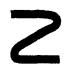
\includegraphics[keepaspectratio]{images/part001_ed0b989f.jpg}}

此外，若 H 是 Riesz 空间（不论是否完全格序），H 中两个元素在 H 中的上确界仍可能不同于它们在 E 中的上确界（习题 3 b)）。最后，还可能发生这样的情形：H 是完全格序的，H 的每个有限子集的上确界在 E 中与在 H 中相同，但存在 H 的在 H 中有上界的无限子集，它们在 E 中与在 H 中的上确界不同（习题 13 f)）。

设 \((\mathrm{E}_{\iota})_{\iota \in \mathrm{I}}\) 是任意一族序向量空间。回顾一下，在积空间 \(\mathrm{E} = \prod_{\iota \in \mathrm{I}}\mathrm{E}_{\iota}\) 中，诸因子空间的序关系的乘积序关系就是关系 \(\ll x_{\iota}\leqslant y_{\iota}\) 对一切 \(\iota \in \mathrm{I}\gg (\mathrm{S},\mathrm{III},\S 1,\mathrm{No.~4})\)。立即可验证这一关系与 E 的向量空间结构相容；赋以这一结构的 E 称为诸序空间 \(E_{\iota}\) 的积空间。

命题 3. --- 设 \((\mathbf{E}_{\iota})_{\iota\in\mathbb{I}}\) 是一族序向量空间。为使积空间 \(E=\prod_{\iota\in I}E_{\iota}\) 是 Riesz 空间（相应地，完全格序空间），必要且充分的是：每个空间 \(E_{\iota}\) 都是 Riesz 空间（相应地，完全格序空间）。

我们只限于考察完全格序空间的情形。设所有 \(E_{\iota}\) 都是完全格序的；设 A 是 E 的一个有上界的非空子集，\(a = (a_{\iota})\) 是 A 的一个上界。对每个 \(\iota \in I\) ，\(pr_{\iota}A\) 以 \(a_{\iota}\) 为上界，因而有上确界 \(b_{\iota}\) （在 \(E_{\iota}\) 中）；显然 \(b = (b_{\iota})\) 是 A 在 E 中的上确界。

反过来，设 E 是完全格序的。设 \(A_{\kappa}\) 是 \(E_{\kappa}\) 的一个有上界的子集，\(A_{\kappa}^{\prime}\) 是 E 中由那些 \(x = (x_{\iota})\) （它们满足 \(x_{\kappa} \in A_{\kappa}\) 且 \(x_{\iota} = 0\) 对 \(\iota \neq \kappa\) ）所组成的子集。立即可以看出 \(A_{\kappa}^{\prime}\) 在 E 中有上界，因而有上确界 \(b = (b_{\iota})\) ；由乘积序关系的定义，必有 \(b_{\iota} = 0\) （对 \(\iota \neq \kappa\) ），而 \(b_{\kappa}\) 是 \(A_{\kappa}\) 的上确界，证毕。

定义 3. --- 设 E 是一个序向量空间，V 与 W 是 E 的两个互补线性子空间。若典范映射 \((x,y)\mapsto x+y\) （把序向量空间 \(V\times W\) 映到序向量空间 E 上）是一个同构，则称 E 是 V 与 W 的序直和。

命题 4. --- 为使序向量空间 E 是两个互补线性子空间 V, W 的序直和，必要且充分的是：关系 \(x \in V\) 、\(y \in W\) 、\(x + y \geqslant 0\) 蕴涵 \(x \geqslant 0\) 与 \(y \geqslant 0\) 。

由于在 E 中 \(x \geqslant 0\) 与 \(y \geqslant 0\) 蕴涵 \(x + y \geqslant 0\) ，命题中的条件表明 \((x, y) \mapsto x + y\) 把由元素 \(\geqslant 0\) 组成的集（取自 \(V \times W\) ）变换为由元素 \(\geqslant 0\) 组成的集（取自 E）。

\subsection{完全格序空间中的带}

定义 4. --- 在完全格序空间 E 中，E 的线性子空间 B 称为一个带，如果它满足以下条件：1) 关系 \(x \in B\) 、\(y \in E\) 与 \(|y| \leqslant |x|\) 蕴涵 \(y \in B\) ；2) 对 B 的每个在 E 中有上界的非空子集 X，X 在 E 中的上确界 sup X 属于 B。

例. --- 在定义在集 A 上的实值函数所成的空间 \(R^{A}\) 中，在 A 的子集 M 的所有点上为零的函数所成的集是一个带。

\pandocbounded{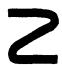
\includegraphics[keepaspectratio]{images/part001_20a85035.jpg}}

注. --- 在空间 \(R^{A}\) 中，A 上有界实值函数所成的子空间 \(\mathcal{B}(A)\) 满足定义 4 的条件 1)；此外，对 \(\mathcal{B}(A)\) 的每个在 \(\mathcal{B}(A)\) 中有上界的子集 X，X 的上包络属于 \(\mathcal{B}(A)\) 。然而，若 A 是无限集，\(\mathcal{B}(A)\) 的一个子集可能在 \(R^{A}\) 中有上界而在 \(\mathcal{B}(A)\) 中没有上界，在这种情形 \(\mathcal{B}(A)\) 不是 \(R^{A}\) 中的带。

由定义 4 立即得出：若 B 是 E 中的一个带，则对 B 的每个在 E 中有下界的非空子集 X，inf X 属于 B。E 中的每个带 B，赋以由 E 诱导的序向量空间结构，都是完全格序空间，且对 B 的每个在 B 中有上界的子集 \(X \subset B\) ，X 在 B 中的上确界与它在 E 中的上确界相同。

完全格序空间 E 中任意一族带的交仍是一个带。对每个子集 \(M \subset E\) ，存在包含 M 的最小带（因为 E 本身就是一个带）；这个带称为由 M 生成的带。

完全格序空间中带的性质以下述命题为基础：

命题 5. --- 设 E 是完全格序空间，A 是 E 的一个由元素 \(\geqslant 0\) 组成的非空子集，满足：1) \(A + A \subset A\) ；2) 关系 \(x \in A\) 、\(0 \leqslant y \leqslant x\) 蕴涵 \(y \in A\) 。设 M 是 A 的那些在 E 中有上界的子集在 E 中的上确界所成的集。在这些条件下，E 的每个元素 \(x \geqslant 0\) 都可写成 \(y + z\) 的形式，其中 \(y \in M\) 是元素 \(v \in A\) （满足 \(v \leqslant x\) 者）的上确界，而 z 是一个与 M 的每个元素互奇异的元素 \(\geqslant 0\) 。

无论如何 \(y \leqslant x\) ，因此问题归结为证明 z = x - y 与每个元素 \(t \in A\) 互奇异 (No. 1)，换句话说，\(u = \inf(z, t)\) 为零。由假设，\(u \in A\) 且 \(u \leqslant x - y\) ，于是 \(u + y \leqslant x\) ；对每个 \(v \in A\) ，若 \(v \leqslant x\) ，则由定义有 \(v \leqslant y\) ，于是 \(u + v \leqslant u + y \leqslant x\) ；由于由假设 \(u + v \in A\) ，由 y 的定义也有 \(u + v \leqslant y\) ；最后，由于 \(u + y\) 是元素 \(u + v\) （其中 \(v \in A\) 且 \(v \leqslant x\) ）在 E 中的上确界，我们有 \(u + y \leqslant y\) ，从而 \(u \leqslant 0\) ，证毕。

定理 1 (F. Riesz). --- 设 A 是完全格序空间 E 的一个子集。与 A 的每个元素互奇异的元素所成的集 A' 是一个带；由与 A' 的每个元素互奇异的元素组成的带 A'\,' 与由 A 生成的带相同，且 E 是诸带 A' 与 A'\,' 的序直和。

在第 1 小节中回顾的互奇异元素的性质以及带的定义立即表明 A' 是一个带，因而 A'\,' 也是一个带。由命题 5 及带的定义，E 的每个元素 \(x \geqslant 0\) 都可写成 \(x = y + z\) ，其中 \(y \in A'\) 且 \(z \in A''\) ，y 与 z 均 \(\geqslant 0\) ；由于 E 的每个元素都是两个 \(\geqslant 0\) 元素之差，我们有 \(E = A' + A''\) ；另一方面，由于 0 是唯一与自身互奇异的元素，我们有 \(A' \cap A'' = \{0\}\) ，这就证明 E 是 \(A'\) 与 \(A''\) 的直和；最后，由于在 \(A'\) 与 \(A''\) 中，E 的元素 \(\geqslant 0\) 的分量都 \(\geqslant 0\) ，E 是 \(A'\) 与 \(A''\) 的序直和 (No. 4, Prop. 4)。

剩下的是要证明 \(A''\) 与由 A 生成的带 B 相同。而 E 是 B 与由和 B 的所有元素互奇异的元素组成的带 \(B'\) 的直和；由于 \(A \subset B\) ，我们有 \(B' \subset A'\) ；另一方面 \(B \subset A''\) ，且 E 也是 \(A'\) 与 \(A''\) 的直和；因此必有 \(B = A''\) ，\(B' = A'\) 。

定理 1 与命题 5 使我们能够给出由 E 的一组元素生成的带的另一个定义：

命题 6. --- 设 E 是完全格序空间，M 是 E 的子集，B 是由 M 生成的带。设 \(M_{1}\) 是 E 中元素 \(\geqslant 0\) 所成的集，其中每个元素都 \(\leqslant\) 某个形如 \(\sum |x_{i}|\) 的元素，这里 \(x_{i} \in M\) ；

设 \(M_{2}\) 是 \(M_{1}\) 的那些有上界的子集的上确界所成的集；则集 \(M_{2}\) 与 B 中元素 \(\geqslant0\) 所成的集相同。

由带的定义，显然 \(M_{2} \subset B\) ；另一方面，若 \(B'\) 是由与 \(M_{1}\) 的每个元素互奇异的元素组成的带，则定理 1 表明 E 是 B 与 \(B'\) 的序直和。而命题 5 表明 E 的每个元素 \(\geqslant 0\) 是 \(M_{2}\) 的一个元素与 \(B'\) 的一个元素之和，由此即得本命题。

推论. --- 设 \(a\) 是完全格序空间 \(\mathbf{E}\) 的一个元素，\(\mathbf{B}_a\) 是由 \(a\) 生成的带，\(\mathbf{B}_a'\) 是与 \(a\) 互奇异的元素所成的带。对每个元素 \(x \geqslant 0\) （属于 \(\mathbf{E}\) ），\(x\) 在 \(\mathbf{B}_a\) 中的分量（相应于把 \(\mathbf{E}\) 分解为 \(\mathbf{B}_a\) 与 \(\mathbf{B}_a'\) 的序直和）等于 \(\sup_{n \in \mathbf{N}} \left( \inf(n|a|, x) \right)\) 。

这由把命题 6 应用于 \(\mathbf{M} = \{a\}\) 以及命题 5 得出。

注意，由 a 与 \(|a|\) 生成的带相同。若 a 与 b 是 E 的两个互奇异元素，且 A 与 B 分别是由 a 与 b 生成的带，则 A 的每个元素与 B 的每个元素互奇异；因为 b 属于由与 a 互奇异的元素组成的带 \(A'\) ，从而 \(B \subset A'\) ，且由定理 1，A 的每个元素与 \(A'\) 的每个元素互奇异。

\section{Riesz 空间上的线性形式}

\subsection{Riesz 空间上的正线性形式}

我们回顾下述定义 (TVS, II, §2, No. 5)：

定义 1. --- 给定一个序向量空间 E，若 E 上的线性形式 L 满足 \(L(x) \geqslant 0\) 对 E 中每个 \(x \geqslant 0\) 成立，则称 L 为正的。

由于 \(L(y) - L(x) = L(y - x)\) ，这等价于说关系 \(x \leqslant y\) 蕴涵 \(L(x) \leqslant L(y)\) ，或者再说一遍，\(L\) 是 \(\mathbf{E}\) 上的递增函数。

例. --- 1) 设 A 是任意集，E 是定义在 A 上的一切实值函数所成的空间 \(R^{A}\) 的一个线性子空间。对每个元素 \(a \in A\) ，映射 \(x \mapsto x(a)\) 是 E 上的一个正线性形式。

\begin{enumerate}
\def\labelenumi{\arabic{enumi})}
\setcounter{enumi}{1}
\item
  设 \(\mathrm{I} = [a, b]\) 是 \(\mathbf{R}\) 中的一个紧区间，\(\mathrm{E}\) 是由 \(\mathrm{I}\) 上的正则实值函数组成的 Riesz 空间 (FRV, II, §1, No. 3)；映射 \(x \mapsto \int_{a}^{b} x(t) dt\) 是 \(\mathrm{E}\) 上的一个正线性形式。
\item
  设 F 是任意集，U 是 F 上的一个超滤子 (GT, I, §6, No. 4)，E 是 F 上有界实值函数所成的 Riesz 空间 \(\mathcal{B}(F)\) 。对每个 \(x \in E\) ，\(\lim_{\mathfrak{U}} x(t)\) 存在，因为 \(x(\mathfrak{U})\) 是相对紧集 \(x(F)\) 上一个超滤子的基，因而收敛。此外，若 \(x \geqslant 0\) ，则由不等式延拓原理，\(\lim_{\mathfrak{U}} x(t) \geqslant 0\) ；于是映射 \(x \mapsto \lim_{\mathfrak{U}} x\) 是 E 上的一个正线性形式。若把 U 取为由包含一个元素 \(a \in F\) 的集合组成的超滤子，就重新得到正线性形式 \(x \mapsto x(a)\) （例 1）。
\end{enumerate}

命题 1. --- 设 E 是序向量空间，L 是 E 到 R 中的一个映射，使得 \(L(x+y)=L(x)+L(y)\) ，且关系 \(x\geqslant0\) 蕴涵 \(L(x)\geqslant0\) ；则 \(L(\lambda x)=\lambda L(x)\) 对每个标量 \(\lambda\) 及每个 \(x\geqslant0\) 成立。

由于 \(L(-x) = -L(x)\) （L 是加群 E 在 R 中的一个表示），我们可以限于 \(\lambda \geqslant 0\) 的情形。对每个整数 \(n \geqslant 0\) ，我们有 \(L(nx) = nL(x)\) ，从而 \(L((1/n)x) = (1/n)L(x)\) ，因而 \(L(rx) = rL(x)\) 对每个有理数 \(r \geqslant 0\) 成立。另一方面，L 在 E 中递增；若 r 与 \(r'\) 是使 \(r \leqslant \lambda \leqslant r'\) 的有理数，则得 \(rL(x) \leqslant L(\lambda x) \leqslant r'L(x)\) ；由于 \(rL(x)\) 与 \(r'L(x)\) 可以任意接近 \(\lambda L(x)\) ，我们有 \(L(\lambda x) = \lambda L(x)\) 。

命题 2. --- 设 E 是实向量空间，C 是 E 中以 0 为顶点的凸锥且 E = C - C，又设 \(x \mapsto M(x)\) 是 C 到 R 中的一个映射，使得 \(M(\lambda x + \mu y) = \lambda M(x) + \mu M(y)\) 对一切 \(x \in C\) 、\(y \in C\) 、\(\lambda \geqslant 0\) 、\(\mu \geqslant 0\) 成立。则存在唯一的线性形式 L 把 M 延拓到 E 上。

由假设，每个 \(z \in E\) 都可写成 \(z = y - x\) ，其中 x, y 属于 C；此外，若又有 \(z = y' - x'\) ，其中 \(x' \in C\) ，\(y' \in C\) ，则

\(M(y) - M(x) = M(y') - M(x')\) ；因为由关系 \(y - x = y' - x'\) 推出 \(y + x' = x + y'\) ，从而 \(M(y) + M(x') = M(x) + M(y')\) 。我们把 \(L(z)\) 定义为 \(M(y) - M(x)\) 当 \(z\) 表为 C 的两元素之差 \(y - x\) 时所取的公共值；立即可以验证，\(L\) 是 E 上延拓 \(M\) 的线性形式；\(L\) 的唯一性由 C 生成空间 E 这一事实得出。

命题 3. --- 设 E 是有向序向量空间，P 是 E 中元素 \(\geqslant 0\) 所成的集，又设 \(x \mapsto M(x)\) 是 P 到 R 中的映射，取值 \(\geqslant 0\) ，使得对 P 中一切 x, y 有 \(M(x + y) = M(x) + M(y)\) 。则存在唯一的正线性形式 L 把 M 延拓到 E 上。

由于 E = P - P，与命题 2 中同样的论证首先证明：存在唯一的 E 到 R 中的加性映射 L 延拓 M。于是命题 1 表明，\(L(\lambda x) = \lambda L(x)\) 对一切 \(\lambda \geqslant 0\) 及一切 \(x \in P\) 成立，由此立即可知 L 是线性形式。

\subsection{相对有界线性形式}

设 E 是有向序向量空间。设 Q 是 E 上正线性形式所成的集；它是 E 的代数对偶 \(E^{*}\) （即 E 上一切线性形式所成的空间）的一个子集。直接可知 \(Q + Q \subset Q\) 且 \(\lambda Q \subset Q\) 对每个标量 \(\lambda > 0\) 成立（换句话说，Q 是 \(E^{*}\) 中的一个凸锥）。此外，\(Q \cap (-Q) = \{0\}\) ，因为若 L 与 -L 都是正线性形式，则 \(L(x) \geqslant 0\) 与 \(L(x) \leqslant 0\) 对一切 \(x \geqslant 0\) 成立，从而 \(L(x) = 0\) 对一切 \(x \geqslant 0\) 成立，因此 L = 0 (No. 1, Prop. 3)。于是集 Q 在 \(E^{*}\) 上定义了一个序关系 \(L \leqslant M\) ，它等价于«M - L 是 E 上的正线性形式»，或者等价于«对每个 \(x \geqslant 0\) ，\(L(x) \leqslant M(x)\) »；对于这个序结构，元素 \(\geqslant 0\) 的 \(E^{*}\) 中的成员就是正线性形式（这证明了所引进术语的合理性）。设 \(\Omega\) 是由 Q 生成的 \(E^{*}\) 的线性子空间，即 E 上作为两个正线性形式之差的线性形式所成的集；当 E 是 Riesz 空间时，我们将给出 \(\Omega\) 的元素的另一个刻划。

定义 2. --- 给定一个 Riesz 空间 E，若对 E 中每个 \(x \geqslant 0\) ，L 在由 \(y \in E\) 中满足 \(|y| \leqslant x\) 者所组成的集上有界，则称 E 上的线性形式 L 为相对有界的。

定理 1. --- \(1^{\circ}\) 为使 Riesz 空间 E 上的线性形式 L 是相对有界的，必要且充分的是：它是两个正线性形式之差。

\(2^{\circ}\) E 上相对有界线性形式所成的序向量空间 \(\Omega\) 是一个完全格序的 Riesz 空间。

若 \(L = U - V\) ，其中 \(U\) 与 \(V\) 是 \(\mathbf{E}\) 上的正线性形式，则关系 \(-x \leqslant y \leqslant x\) 蕴涵

\[
- U (x) \leqslant U (y) \leqslant U (x) \quad \text { and } \quad - V (x) \leqslant V (y) \leqslant V (x),
\]

由此立即可得 \(|L(y)| \leqslant U(x) + V(x)\) ；于是 L 是相对有界的。反过来，设 L 是相对有界的；问题归结为证明存在一个正线性形式 N，使 \(N(x) \geqslant L(x)\) 对一切 \(x \geqslant 0\) 成立，因为这时 N - L 将是一个正线性形式。

而若一个正线性形式 N 具有这一性质，则对每个 \(x \geqslant 0\) 及 \(0 \leqslant y \leqslant x\) ，我们有 \(N(x) \geqslant N(y) \geqslant L(y)\) ，因此 \(N(x) \geqslant \sup_{0 \leqslant y \leqslant x} L(y)\) ；若我们能证明实值函数

\[
x \mapsto M (x) = \sup _ {0 \leqslant y \leqslant x} L (y),
\]

（它定义在 E 中元素 \(\geqslant0\) 所成的集 P 上）可以延拓为 E 上的一个正线性形式（仍记作 M），则我们就证明了定理的第一部分，并且还证明了 M 是 \(\Omega\) 中 0 与 L 的上确界。由于在 P 上 \(M(x)\geqslant0\) ，问题归结为证明

\[
M (x + x ^ {\prime}) = M (x) + M (x ^ {\prime})
\]

对 E 的每对元素 \(x \geqslant 0\) 、\(x' \geqslant 0\) 成立 (No. 1, Prop. 3)。由定义，

\[
\begin{array}{c} M (x) + M (x ^ {\prime}) = \sup _ {0 \leqslant y \leqslant x} L (y) + \sup _ {0 \leqslant y ^ {\prime} \leqslant x ^ {\prime}} L (y ^ {\prime}) \\ = \sup _ {0 \leqslant y \leqslant x, 0 \leqslant y ^ {\prime} \leqslant x ^ {\prime}} L (y + y ^ {\prime}) \leqslant M (x + x ^ {\prime}). \end{array}
\]

另一方面，对每个 \(z\) （它满足 \(0 \leqslant z \leqslant x + x'\) ），我们有 \(x + x' = z + u\) ，其中 \(u \geqslant 0\) ；由分解引理 (§1, No. 1)，存在两个元素 \(y, y'\) ，使得 \(0 \leqslant y \leqslant x\) 、\(0 \leqslant y' \leqslant x'\) ，且 \(z = y + y'\) ，\(u = (x - y) + (x' - y')\) ；于是

\[
L (z) = L (y) + L \left(y ^ {\prime}\right) \leqslant M (x) + M \left(x ^ {\prime}\right),
\]

因此 \(M(x + x') = \sup_{0 \leqslant z \leqslant x + x'} L(z) \leqslant M(x) + M(x')\) ，这就完成了定理第一部分的证明。此外，我们这样还证明了 \(\Omega\) 是一个 Riesz 空间，并且对 E 上每个相对有界线性形式 L 及每个 \(x \geqslant 0\) ，

\[
L ^ {+} (x) = \sup _ {0 \leqslant y \leqslant x} L (y).\tag{1}
\]

剩下的是要看出 \(\Omega\) 是完全格序的；为此，只需证明正线性形式的任何有上界且依关系 \(\leqslant\) 有向的集 H 在 \(\Omega\) 中有一个上确界。

更一般地，我们有下述引理：

引理. --- 设 E 是有向序向量空间，\(E^{*}\) 是它的对偶，以正线性形式为正元素而排序。设 \((u_{\alpha})\) 是 \(E^{*}\) 中元素的一个递增有向族。若对 E 中每个 \(x \geqslant 0\) ，\(\sup u_{\alpha}(x) < +\infty\) ，则族 \((u_{\alpha})\) 在 \(E^{*}\) 中有一个上确界 u，且对 E 中一切 \(x \geqslant 0\) ，

\[
u (x) = \sup _ {\alpha} u _ {\alpha} (x).\tag{2}
\]

在 E 中一切 \(x \geqslant 0\) 所成的集 P 上，用公式 (2) 定义映射 u；直接可知，\(u(\lambda x) = \lambda u(x)\) 对一切 \(\lambda \geqslant 0\) 及 \(x \in P\) 成立；因此，由 No. 1 的命题 2，为证明本引理，只需证明

\[
u (x + y) = u (x) + u (y)
\]

对 P 中的 \(x, y\) 成立。但只要注意到，关于指标的定向集，\(u(x) = \lim u_{\alpha}(x)\) （单调极限定理），这就立即可得。

由公式 (1) 立即推出：若 L 与 M 是 E 上两个相对有界线性形式，则对每个 \(x \geqslant 0\) ，

\[
\left\{ \begin{array}{l} \sup (L, M) (x) = \sup _ {y \geqslant 0,   z \geqslant 0,   y + z = x} \big (L (y) + M (z) \big) \\ \inf (L, M) (x) = \inf _ {y \geqslant 0,   z \geqslant 0,   y + z = x} \big (L (y) + M (z) \big). \end{array} \right.\tag{3}
\]

特别地，若在这些公式的第一个中把 \(M\) 换成 \(-L\) ，就得到

\[
| L | (x) = \sup _ {y \geqslant 0, z \geqslant 0, y + z = x} L (y - z).
\]

而若 \(x = y + z\) 、\(y \geqslant 0\) 且 \(z \geqslant 0\) ，则 \(-x \leqslant y - z \leqslant x\) ；反过来，关系 \(|u| \leqslant x\) 蕴涵 \(L(u) \leqslant |L|(|u|) \leqslant |L|(x)\) 。由此我们导出公式

\[
| L | (x) = \sup _ {| y | \leqslant x} L (y) \quad \text { for } x \geqslant 0,\tag{4}
\]

从而特别有，

\[
| L (x) | \leqslant | L | (| x |)\tag{5}
\]

对一切 \(x \in \mathbf{E}\) 成立。

命题 4. --- 为使 Riesz 空间 E 上两个正线性形式 L, M 在空间 \(\Omega\) 中互奇异，必要且充分的是：对每个数 \(\varepsilon > 0\) 及 E 中每个 \(x \geqslant 0\) ，存在 E 的两个元素 \(y \geqslant 0\) 、\(z \geqslant 0\) ，使得 \(x = y + z\) 且 \(L(y) + M(z) \leqslant \varepsilon\) 。事实上，由 (3) 中第二个公式，这一条件表示 \(\inf(L, M) = 0\) 。

命题 5. --- 设 L 是 Riesz 空间 E 上的一个正线性形式。为使 E 上的正线性形式 M 属于 \(\Omega\) 中由 L 生成的带，必要且充分的是：对 E 中每个 \(x \geqslant 0\) 及每个数 \(\varepsilon > 0\) ，存在一个数 \(\delta > 0\) ，使得关系 \(0 \leqslant y \leqslant x\) 与 \(L(y) \leqslant \delta\) 蕴涵 \(M(y) \leqslant \varepsilon\) 。

我们先证明条件是必要的。若 \(M \geqslant 0\) 属于 \(\Omega\) 中由 L 生成的带，则 (§1, No. 5, Prop. 6 的推论)

\[
M = \sup _ {n} \left(\inf (n L, M)\right).
\]

若令

\[
U _ {n} = M - \inf (n L, M),
\]

于是 \(U_{n}\) 是 E 上的一个正线性形式，且 \(\inf_{n} U_{n} = 0\) 在 \(\Omega\) 中成立；因而（引理）当 n 趋于无穷时 \(U_{n}(x)\) 趋于 0，且存在 n 使 \(U_{n}(x) \leqslant \varepsilon / 2\) 。固定这样一个 n，则 \(U_{n}(y) \leqslant \varepsilon / 2\) 对一切满足 \(0 \leqslant y \leqslant x\) 的 y 成立，于是关系 \(0 \leqslant y \leqslant x\) 蕴涵

\[
M (y) \leqslant \frac {\varepsilon}{2} + \inf (n L, M) (y) \leqslant \frac {\varepsilon}{2} + n L (y);
\]

若 \(y\) 使 \(L(y) \leqslant \varepsilon / 2n\) ，则得 \(M(y) \leqslant \varepsilon\) ，这就证明了我们的断言。

现在证明条件是充分的。设 \(M\) 是 \(\mathrm{E}\) 上任一正线性形式，则可写 \(M = U + V\) ，其中 \(U\) 属于由 \(L\) 在 \(\Omega\) 中生成的带，而 \(V\) 与 \(L\) 互奇异，\(U\) 与 \(V\) 都是正的 (§1, No. 5, Th. 1)。若 \(M\) 满足命题中的条件，则 \(V = M - U\) 也满足，因为 \(0 \leqslant V \leqslant M\) 。由此我们将推出 \(V = 0\) 。对每个 \(x \geqslant 0\) （在 \(\mathrm{E}\) 中）及每个数 \(\eta > 0\) ，存在两个元素 \(y \geqslant 0\) 、\(z \geqslant 0\) （属于 \(\mathrm{E}\)），使得 \(x = y + z\) 且 \(L(y) + V(z) \leqslant \eta\) （命题 4）；给定任意数 \(\varepsilon > 0\) ，选取 \(\eta \leqslant \varepsilon\) ，使得关系 \(0 \leqslant u \leqslant x\) 与 \(L(u) \leqslant \eta\) 蕴涵 \(V(u) \leqslant \varepsilon\) ；把 \(y\) 与 \(z\) 取定如上，我们有 \(L(y) \leqslant \eta\) ，因此 \(V(y) \leqslant \varepsilon\) ，于是

\[
V (x) = V (y) + V (z) \leqslant \varepsilon + \eta \leqslant 2 \varepsilon ;
\]

由于 \(\varepsilon\) 是任意的，我们有 \(V(x) = 0\) 对每个 \(x \geqslant 0\) 成立，即 \(V = 0\) 。

例. --- 设 E 是一个 Riesz 空间，赋以一个与其序向量空间结构相容的局部凸拓扑 (TVS, II, §2, No. 7)。设 \(E'\) 是 E 的拓扑对偶，并再设 E 中元素 \(\geqslant 0\) 所成的锥 P 对于弱化拓扑 \(\sigma(\mathrm{E},\mathrm{E}')\) 是完备的。则每个连续线性形式 \(x' \in E'\) 都是相对有界的，因为已知 (TVS, II, §6, No. 8, Prop. 11 的推论 2)，在这些条件下，对 E 中每个 \(x \geqslant 0\) ，由 \(y \in E\) 中满足 \(|y| \leqslant x\) 者所成的集对 \(\sigma(\mathrm{E},\mathrm{E}')\) 是紧的。由此我们推出 E 这时是完全格序的；因为 (§1, No. 3, Prop. 2)，只需证明：对每个集 \(H \subset E\) （它有上界且依 \(\leqslant\) 有向），H 的截断滤子 F 在 E 中对拓扑 \(\sigma(\mathrm{E},\mathrm{E}')\) 收敛（后者与 E 的序向量空间结构相容）。由平移，我们可以假设 \(H \subset P\) ，于是只需证明 F 是对 \(\sigma(\mathrm{E},\mathrm{E}')\) 的 Cauchy 滤子，或者再说一遍，每个连续线性形式 \(x' \in E'\) 关于 F 有极限。而当 \(x'\) 是正线性形式时，这由单调极限定理立即可得；又由于每个线性形式 \(x' \in E'\) 是两个正线性形式之差 (Th. 1)，我们的断言得证。
